\problemname{Chasing Rats}

\noindent
Last year, no one managed to drive the giant rats out of Gothenburg (see the problem \textit{KATT:s and rats}\footnote{\url{https://open.kattis.com/problems/rats2}}).
Because of this, Olle has no choice but to take matters into his own hands and personally chase all of Gothenburg's rats into traps.

Gothenburg's sewers consist of $N$ manholes, and there are $M$ pipes connecting pairs of manholes.
When Olle chases a rat, he places a trap in manhole $T$. He starts in manhole $S$, and the rat starts in manhole $R$.
The goal is to get the rat to enter the trap in manhole $T$. Olle can move between manholes using the pipes.
If he enters the same manhole as the rat, the rat will flee to an adjacent manhole.
After chasing many rats, he has noticed that they are predictable: if he enters a manhole from a certain pipe,
the rat will always flee to a specific manhole.

Unfortunately, Olle has noticed that some rats cannot be caught.
He therefore needs your help $Q$ times to determine whether it is possible to capture the rat given $S, R$, and $T$.
All queries are independent of each other, and there is always exactly one rat in the sewers per query.

\section*{Input}
The first line of input contains the integers $N, M,$ and $Q$ ($3 \leq N \leq 10^5$, $1 \le M,Q \le 10^5$),
the number of manholes, the number of pipes, and the number of queries.

The next $M$ lines each describe a pipe. Each pipe is described by the integers $u,v,a,b$
($1 \leq u,v,a,b \leq N$, $u \neq v$), where $u,v$ indicate that there is a pipe between manholes $u$ and $v$.
$a$ specifies that if Olle travels from $u$ to $v$ and a rat is in manhole $v$, it will flee to manhole $a$.
$b$ similarly specifies that if Olle is in manhole $v$ and travels to $u$, the rat will flee to manhole $b$.
It is also guaranteed that there is at most one pipe between each pair of manholes,
the pipe $(v,a)$ exists, the pipe $(u,b)$ exists It is possible for Olle to travel between any two manholes.

Then follows $Q$ lines, each containing the integers $S, R, T$ ($1 \leq S,R,T \leq N$),
describing that Olle wonders whether he can chase the rat in manhole $R$ to manhole $T$ if he starts in manhole $S$.
It is guaranteed that $T\neq S$, $T\neq R$, and $S\neq R$.

\textbf{Note} that this problem has a very large input size. Therefore, it is recommended to use fast input reading.

\section*{Output}
Answer each query in the same order as the input. If Olle can chase the rat into the trap, print
\texttt{1}, otherwise print \texttt{0}.

\section*{Scoring}
Your solution will be tested on a set of test groups, each worth a number of points. Each test group contains
a set of test cases. To get the points for a test group you need to solve all test cases in the test group.

Let $deg(u)$ be the number of pipes that connect to manhole $u$.

\noindent
\begin{tabular}{| l | l | p{12cm} |}
  \hline
  \textbf{Group} & \textbf{Points} & \textbf{Constraints} \\ \hline
  $1$    & $5$        & $N, M \leq 50, Q \leq 100$ \\ \hline
  $2$    & $11$       & $N, M \leq 500, Q \leq 10000$ \\ \hline
  $3$    & $20$       & $Q=1$, $deg(u) \leq 5$ for all $1 \leq u \leq N$. \\ \hline
  $4$    & $23$       & $Q=1$ \\ \hline
  $5$    & $12$       & $S$ and $R$ are the same for all queries. \\ \hline
  $6$    & $17$       & $T$ is the same for all queries. \\ \hline
  $7$    & $10$       & $N, M \leq 30000$ \\ \hline
  $8$    & $2$        & No additional constraints. \\ \hline
\end{tabular}

\section*{Explanation of Samples}

The manholes are connected as follows. The escape routes for the rat are not drawn to reduce clutter.

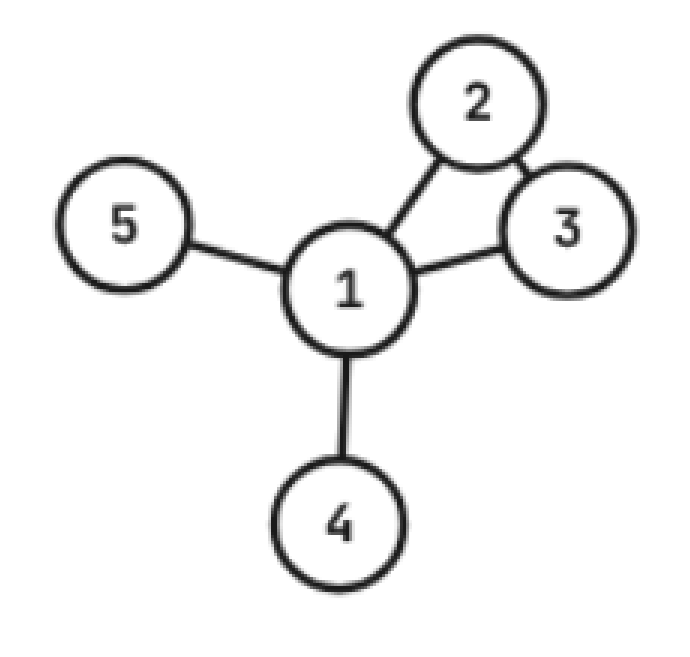
\includegraphics[scale=0.5]{sample}  

\begin{itemize}
  \item Question 1: There is no escape route for the rat that leads to manhole 4. Therefore, the answer is no.  
  \item Question 2: Olle can chase the rat into the trap directly.  
  \item Question 3: No matter how Olle chases the rat, he can never reach manhole 4 while the rat is in manhole 1. Therefore, the answer is no.  
\end{itemize}
